\section{Internal Tests}

\subsection{GOAL Test Set}

\subsubsection{Timeouts and Memory Excesses}

Timeout for each complementation task: 600 seconds CPU time. Memory limit by limiting Java heap to 1 GB.

\begin{table}[ht]
\centering
\begin{tabular}{lrr}
  \hline
Construction & Time & Memory \\ 
  \hline
Fribourg & 48 & 0 \\ 
  Fribourg+R2C & 30 & 0 \\ 
  Fribourg+R2C+C & 54 & 0 \\ 
  Fribourg+M1 & 2 & 0 \\ 
  Fribourg+M1+M2 & 1 & 0 \\ 
  Fribourg+M1+R2C & 1 & 0 \\ 
  Fribourg+M1+R2C+C & 8 & 0 \\ 
  Fribourg+R & 24 & 0 \\ 
   \hline
\end{tabular}
\caption{Number of timeouts and memory excesses.}
\end{table}


The number of effective samples is 10,939. That is, 10,939 of the 11,000 automata have been successfully complemented by all constructions, while 61 automata have failed to complement with at least one of the constructions.

\textcolor{red}{It is strange that Fribourg+R has so much fewer timeouts than Fribourg}

\begin{figure}[ht]
\centering
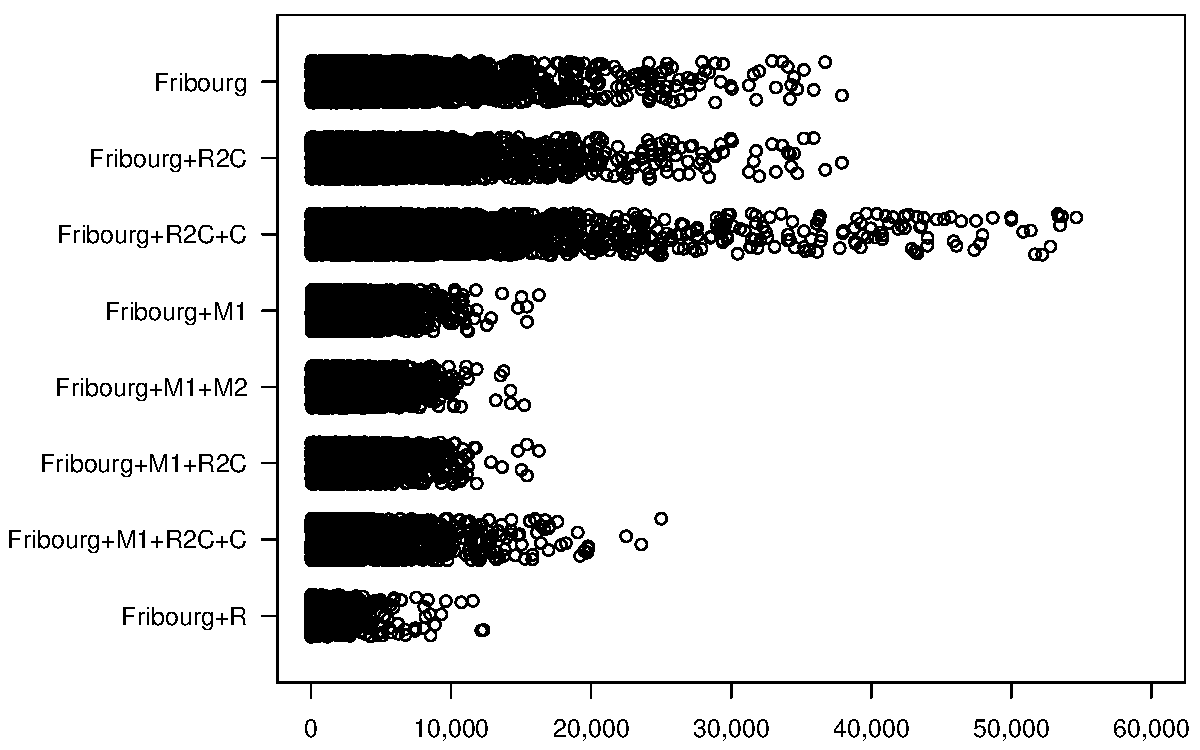
\includegraphics[width=0.75\textwidth]{figures/r/internal/goal/stripchart.pdf}
\caption{Number of states of complements.}
\end{figure}


\subsubsection{Statistics Aggregated}

Number of states of the produced complement automaton, aggregated over the whole test set.

\begin{table}[ht]
\centering
\begin{tabular}{lrrrrrr}
  \hline
Construction & Mean & Min. & P25 & Median & P75 & Max. \\ 
  \hline
Fribourg & 2,004.6 & 2 & 222.0 & 761.0 & 2,175.0 & 37,904 \\ 
  Fribourg+R2C & 1,955.9 & 2 & 180.0 & 689.0 & 2,127.5 & 37,904 \\ 
  Fribourg+R2C+C & 2,424.6 & 2 & 85.0 & 451.0 & 2,329.0 & 54,648 \\ 
  Fribourg+M1 & 963.2 & 2 & 177.0 & 482.0 & 1,138.0 & 16,260 \\ 
  Fribourg+M1+M2 & 958.0 & 2 & 181.0 & 496.0 & 1,156.5 & 15,223 \\ 
  Fribourg+M1+R2C & 937.7 & 2 & 152.0 & 447.0 & 1,118.0 & 16,260 \\ 
  Fribourg+M1+R2C+C & 1,062.6 & 2 & 83.0 & 331.0 & 1,208.5 & 25,002 \\ 
  Fribourg+R & 136.3 & 1 & 1.0 & 1.0 & 21.0 & 12,312 \\ 
   \hline
\end{tabular}
\caption{Aggregated statistics.}
\end{table}

Statistics over the execution time in CPU time of all the automata.

\begin{table}[ht]
\centering
\begin{tabular}{lrrrrrr}
  \hline
Construction & Mean & Min. & P25 & Median & P75 & Max. \\ 
  \hline
Fribourg & 8.53 & 2.49 & 3.30 & 4.89 & 7.26 & 585.99 \\ 
  Fribourg+R2C & 6.63 & 2.19 & 2.86 & 4.18 & 6.40 & 219.68 \\ 
  Fribourg+R2C+C & 8.54 & 2.16 & 2.56 & 3.48 & 6.38 & 582.87 \\ 
  Fribourg+M1 & 4.94 & 2.47 & 3.16 & 4.10 & 5.85 & 55.07 \\ 
  Fribourg+M1+M2 & 4.56 & 2.21 & 2.89 & 3.78 & 5.11 & 38.43 \\ 
  Fribourg+M1+R2C & 4.44 & 2.22 & 2.83 & 3.59 & 5.27 & 42.48 \\ 
  Fribourg+M1+R2C+C & 5.57 & 2.51 & 3.23 & 3.97 & 6.51 & 147.44 \\ 
  Fribourg+R & 6.00 & 2.15 & 2.71 & 3.58 & 5.70 & 166.57 \\ 
   \hline
\end{tabular}
\caption{Running times in seconds of the complementation tasks, measured as CPU time.}
\end{table}

\textcolor{red}{It is strange that Fribourg+R is so much faster than Fribourg}

\subsubsection{Statistics Split Up by dt/da classes}

\newcommand{\perspwidth}{0.475}

\begin{figure}[ht]
\centering
  \hfill
  \begin{subfigure}[t]{\perspwidth\textwidth}
  \centering
  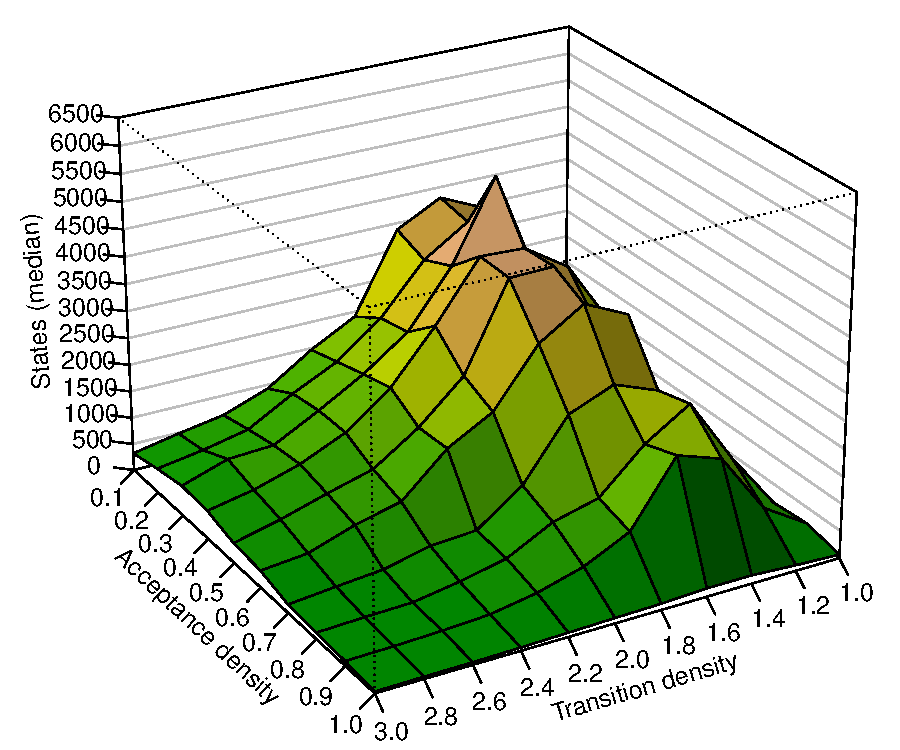
\includegraphics[width=\textwidth]{figures/r/internal/goal/s.median.Fribourg.pdf}
  \caption{Fribourg}
  \end{subfigure}
  \hfill
  \begin{subfigure}[t]{\perspwidth\textwidth}
  \centering
  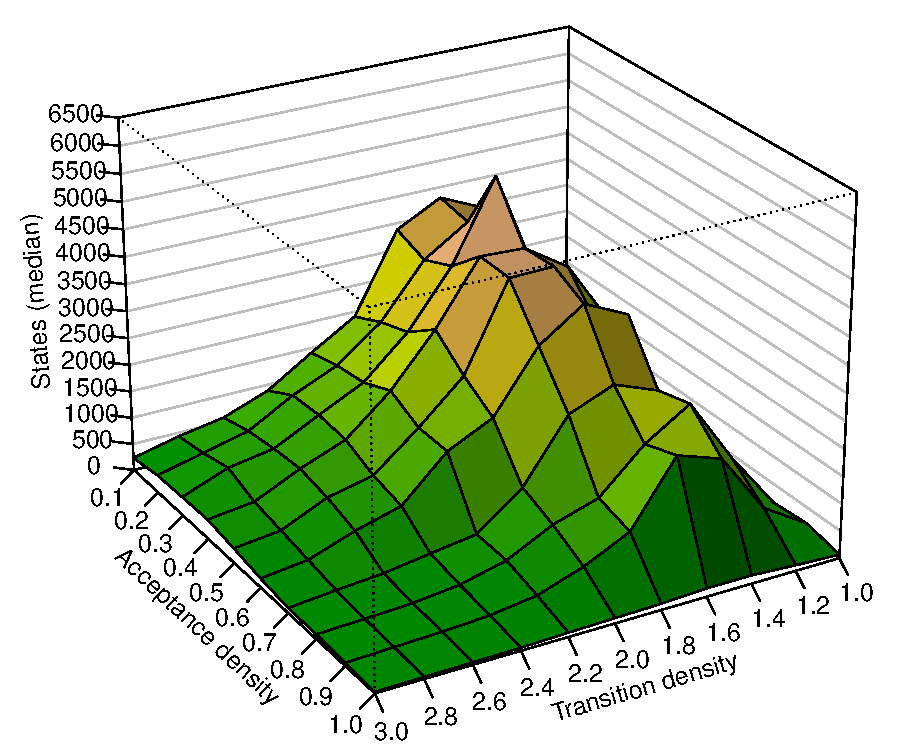
\includegraphics[width=\textwidth]{figures/r/internal/goal/s.median.Fribourg+R2C.pdf}
  \caption{Fribourg+R2C}
  \end{subfigure}
  \hfill

  \hfill
  \begin{subfigure}[t]{\perspwidth\textwidth}
  \centering
  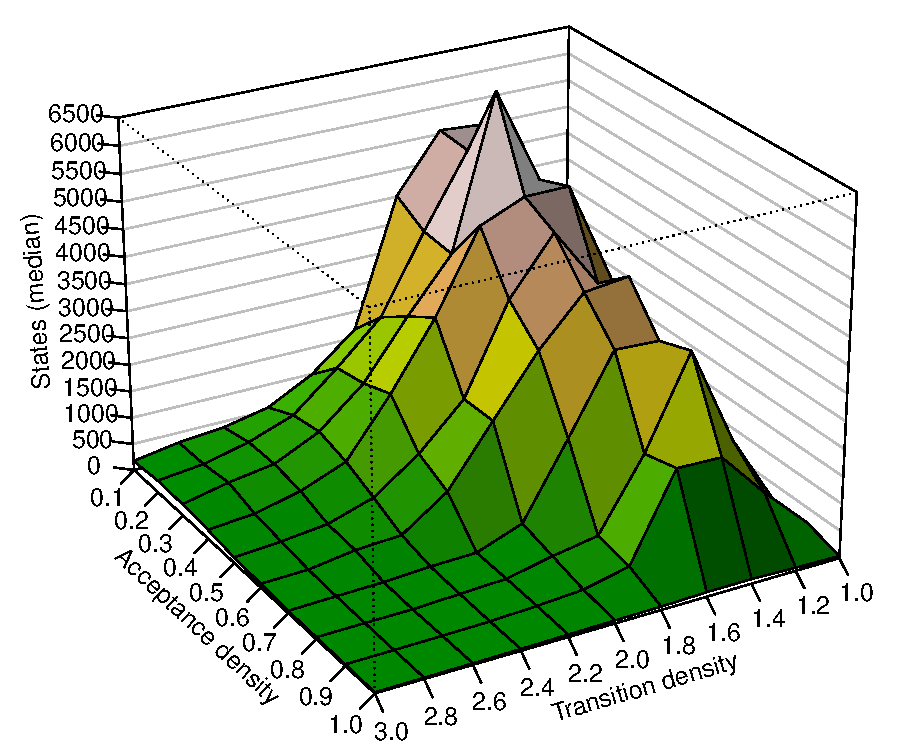
\includegraphics[width=\textwidth]{figures/r/internal/goal/s.median.Fribourg+R2C+C.pdf}
  \caption{Fribourg+R2C+C}
  \end{subfigure}
  \hfill
  \begin{subfigure}[t]{\perspwidth\textwidth}
  \centering
  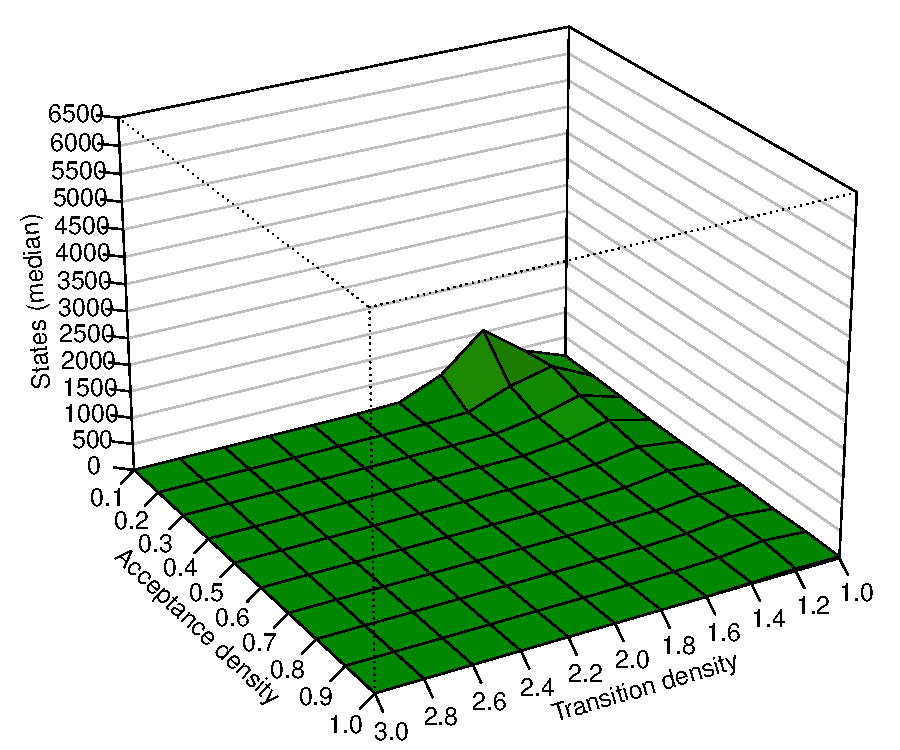
\includegraphics[width=\textwidth]{figures/r/internal/goal/s.median.Fribourg+R.pdf}
  \caption{Fribourg+R}
  \end{subfigure}
  \hfill  
\caption{Median states}
\end{figure}

\begin{figure}[ht]
\centering
  \hfill
  \begin{subfigure}[t]{\perspwidth\textwidth}
  \centering
  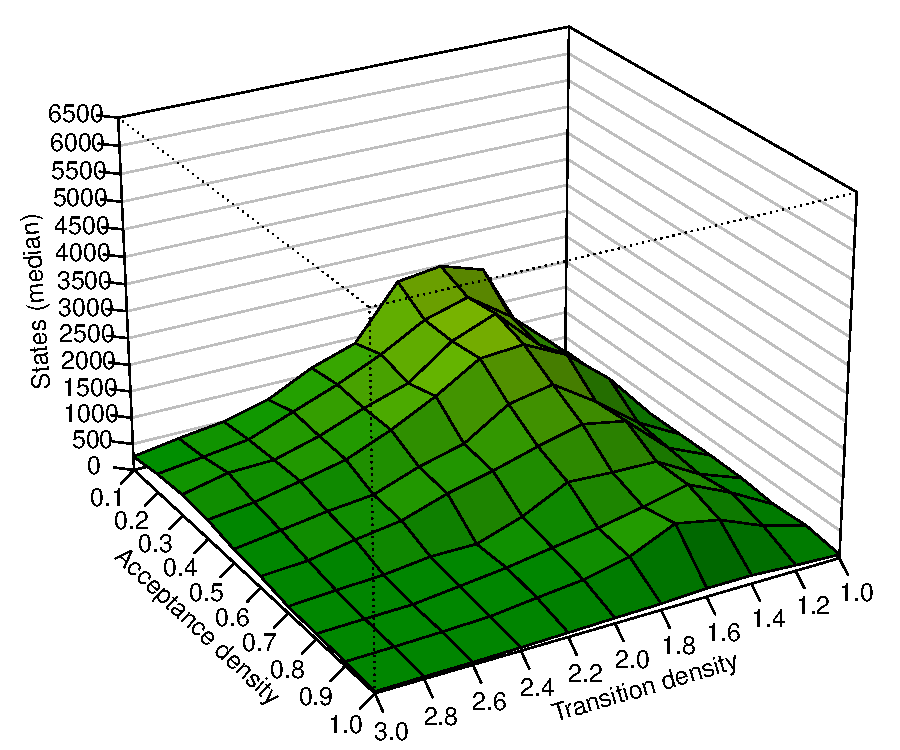
\includegraphics[width=\textwidth]{figures/r/internal/goal/s.median.Fribourg+M1.pdf}
  \caption{Fribourg+M1}
  \end{subfigure}
  \hfill
  \hfill
  \begin{subfigure}[t]{\perspwidth\textwidth}
  \centering
  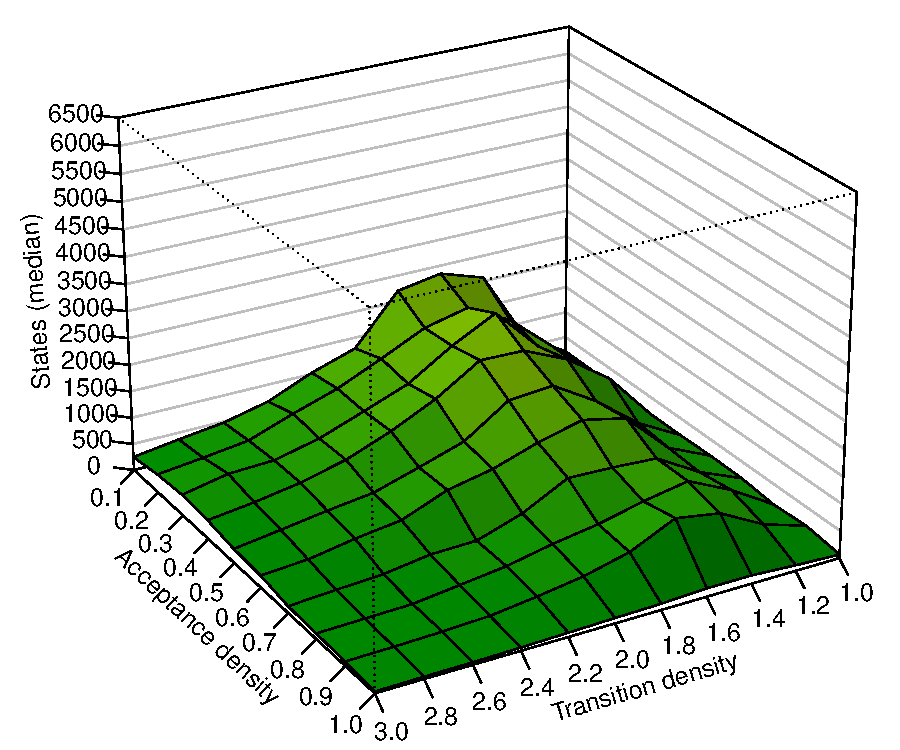
\includegraphics[width=\textwidth]{figures/r/internal/goal/s.median.Fribourg+M1+M2.pdf}
  \caption{Fribourg+M1+M2}
  \end{subfigure}
  \hfill

  \hfill
  \begin{subfigure}[t]{\perspwidth\textwidth}
  \centering
  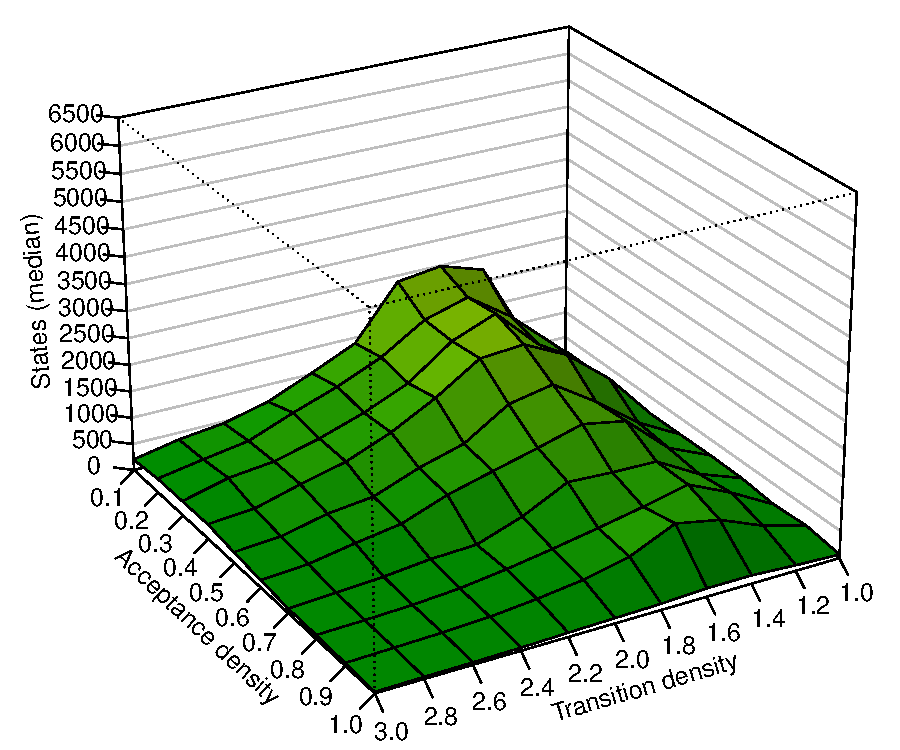
\includegraphics[width=\textwidth]{figures/r/internal/goal/s.median.Fribourg+M1+R2C.pdf}
  \caption{Fribourg+M1+R2C}
  \end{subfigure}
  \hfill
  \begin{subfigure}[t]{\perspwidth\textwidth}
  \centering
  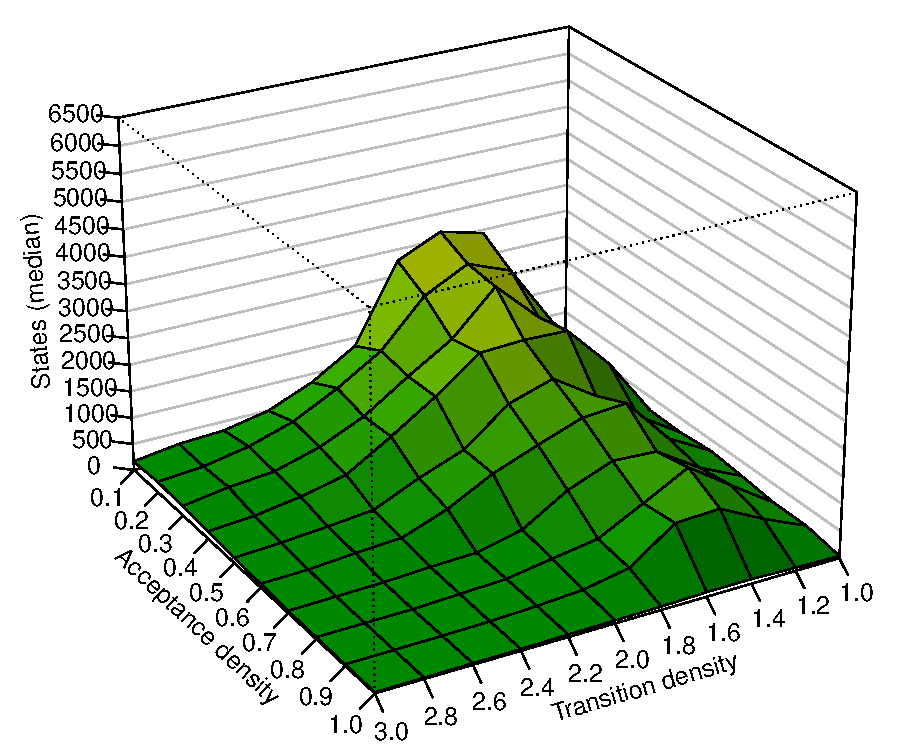
\includegraphics[width=\textwidth]{figures/r/internal/goal/s.median.Fribourg+M1+R2C+C.pdf}
  \caption{Fribourg+M1+R2C+C}
  \end{subfigure}
  \hfill
\end{figure}

\subsubsection{Difficulty Classes of the GOAL Test Set}

\begin{figure}[ht]
\centering
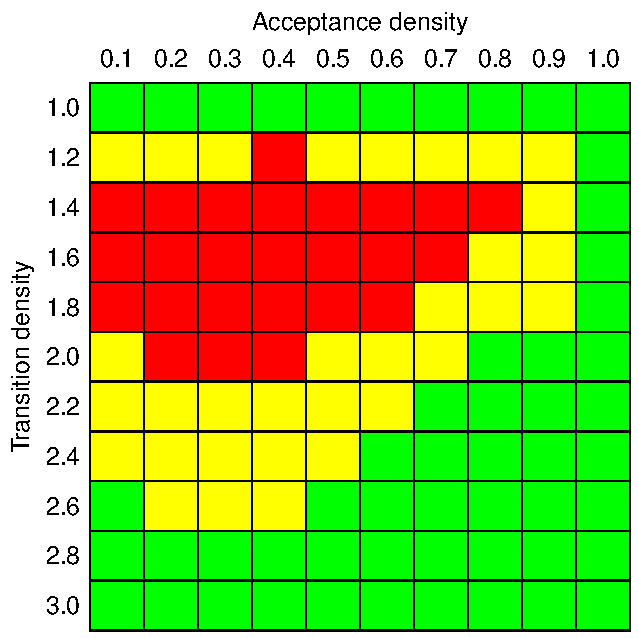
\includegraphics[width=0.4\textwidth]{figures/r/internal/goal/s.median.image.pdf}
\caption{Average of the median number of produced states of all the constructions: green (easy): $\leq$ 500; yellow (medium): $\leq$ 1450; red (hard): $>$ 1450.}
\end{figure}



\subsection{Michel Automata}
Michel automata are complete, thus the C options makes no sense.

For the Michel automata Fribourg+M1+M2 is better than Fribourg+M1. Fribourg+M1+R2C is again much better than Fribourg+M1 and even Fribourg+M1+M2. Thus, we have to test Fribourg+M1+M2+R2C. 

\begin{itemize}
\item Add Fribourg+M1+M2+R2C
\item Add Fribourg+M1+M2+R2C+R
\item Add Fribourg+R
\end{itemize}



\begin{tabular}{r|rrrrrrrrrr}
  \hline
 & 0.1 & 0.2 & 0.3 & 0.4 & 0.5 & 0.6 & 0.7 & 0.8 & 0.9 & 1.0 \\ 
  \hline
1.0 & 580.3 & 465.0 & 786.4 & 401.2 & 398.4 & 300.3 & 336.7 & 263.3 & 297.4 & 77.3 \\ 
  1.2 & 1730.8 & 2050.2 & 1780.7 & 1808.5 & 1328.1 & 1298.1 & 1421.8 & 1108.0 & 987.4 & 136.4 \\ 
  1.4 & 3409.1 & 3251.7 & 2471.2 & 3052.9 & 2210.9 & 2255.1 & 1638.0 & 1437.3 & 1561.8 & 172.0 \\ 
  1.6 & 3493.9 & 3280.5 & 3395.7 & 3005.0 & 2215.7 & 1921.1 & 1599.5 & 1418.9 & 1401.5 & 170.3 \\ 
  1.8 & 2714.1 & 2418.7 & 2677.5 & 2199.3 & 2102.1 & 1689.1 & 1367.8 & 876.0 & 842.8 & 127.3 \\ 
  2.0 & 1778.3 & 1961.6 & 1769.2 & 1805.8 & 1401.0 & 1275.3 & 803.5 & 682.4 & 510.7 & 107.8 \\ 
  2.2 & 1180.9 & 1498.6 & 1257.8 & 1219.9 & 989.9 & 926.0 & 519.3 & 412.0 & 314.4 & 82.6 \\ 
  2.4 & 719.6 & 992.4 & 1036.3 & 848.8 & 659.2 & 615.9 & 388.6 & 287.8 & 195.4 & 60.8 \\ 
  2.6 & 553.0 & 682.8 & 673.3 & 660.3 & 555.1 & 483.2 & 265.0 & 190.2 & 153.2 & 49.1 \\ 
  2.8 & 454.6 & 490.5 & 609.6 & 489.8 & 419.2 & 336.3 & 222.7 & 154.1 & 118.9 & 41.1 \\ 
  3.0 & 276.4 & 381.4 & 403.5 & 390.1 & 323.8 & 255.3 & 136.2 & 119.5 & 82.2 & 35.0 \\ 
   \hline
\end{tabular}

asdflkjasdf


asdflkjf

\begin{tabular}{r|rrrrrrrrrr}
 & 0.1 & 0.2 & 0.3 & 0.4 & 0.5 & 0.6 & 0.7 & 0.8 & 0.9 & 1.0 \\ 
  \hline
1.0 & 269.0 & 308.0 & 254.0 & 236.0 & 238.5 & 297.0 & 266.0 & 156.0 & 207.0 & 68.0 \\ 
  1.2 & 960.0 & 1,407.5 & 1,479.0 & 2,150.0 & 1,152.0 & 1,090.5 & 942.5 & 1,206.5 & 718.0 & 104.5 \\ 
  1.4 & 3,426.0 & 2,915.0 & 2,752.0 & 3,393.0 & 2,693.0 & 3,265.5 & 2,263.5 & 2,425.0 & 1,844.5 & 154.5 \\ 
  1.6 & 3,799.0 & 3,698.0 & 4,901.5 & 3,926.0 & 3,960.0 & 3,655.0 & 2,580.5 & 1,905.5 & 2,124.5 & 155.0 \\ 
  1.8 & 3,375.0 & 3,169.0 & 3,420.5 & 3,967.0 & 3,943.0 & 3,132.0 & 2,246.5 & 1,144.0 & 971.5 & 114.0 \\ 
  2.0 & 1,906.5 & 2,261.0 & 2,383.0 & 2,884.0 & 2,354.5 & 2,096.5 & 1,169.5 & 932.0 & 568.0 & 98.5 \\ 
  2.2 & 1,467.0 & 1,633.0 & 1,795.5 & 1,942.5 & 1,611.5 & 1,640.5 & 569.5 & 499.0 & 330.5 & 78.5 \\ 
  2.4 & 924.5 & 1,232.5 & 1,319.0 & 1,317.5 & 1,056.5 & 886.5 & 514.5 & 314.5 & 182.0 & 59.0 \\ 
  2.6 & 625.0 & 763.0 & 880.5 & 945.5 & 828.0 & 684.5 & 316.0 & 175.0 & 132.0 & 44.5 \\ 
  2.8 & 483.5 & 584.5 & 836.0 & 690.0 & 575.0 & 395.5 & 240.0 & 151.5 & 103.0 & 41.0 \\ 
  3.0 & 319.5 & 450.5 & 557.0 & 523.5 & 367.5 & 313.5 & 155.5 & 116.0 & 84.5 & 32.0 \\ 
\end{tabular}

\begin{tabular}{lrrrrrr}
  \hline
Version & Mean & Min & P25 & Median & P75 & Max \\ 
  \hline
fribourg.goal & 2,004.57 & 2 & 222.00 & 761.00 & 2,175.00 & 37,904 \\ 
  fribourg.m1.goal & 963.17 & 2 & 177.00 & 482.00 & 1,138.00 & 16,260 \\ 
  fribourg.m1.m2.goal & 958.00 & 2 & 181.00 & 496.00 & 1,156.50 & 15,223 \\ 
  fribourg.m1.r2c.goal & 937.66 & 2 & 152.00 & 447.00 & 1,118.00 & 16,260 \\ 
  fribourg.m1.r2c.macc.r.goal & 115.40 & 1 & 1.00 & 1.00 & 20.00 & 9,843 \\ 
  fribourg.r2c.c.goal & 2,424.56 & 2 & 85.00 & 451.00 & 2,329.00 & 54,648 \\ 
  fribourg.r2c.goal & 1,955.91 & 2 & 180.00 & 689.00 & 2,127.50 & 37,904 \\ 
   \hline
\end{tabular}



\section{External Tests}

\subsection{GOAL Test Set}

With \em{rank -tr -ro} there are 3796 uncompleted tasks (7,204 effective samples), without it only 7 (10,993 effective samples). Should the main analysis be done without rank? Because of rank, we would exclude the most difficult cases for the other constructions from the analysis.

With \em{piterman -eq -sim -ro}, the median is 1 and the 75th percentile 21. It' similar as when removing unreachable and dead states from the output automaton. I think this is caused by the sim optimisation, which simplifies one of the intermediate automata of the construction. Have to try the following:

\begin{itemize}
\item piterman -eq -sim -ro -r
\item piterman -eq -ro
\end{itemize}
